\section{Evaluations}\label{sec:eval}
\begin{figure}[!t]
\resizebox{\linewidth}{!}{
\begin{tikzpicture}

\def\barone{0.2}
\def\bartwo{0.6}
\def\barthree{1.2}
\def\barfour{3.1}
\def\barfive{4.2}
\def\barsix{6.1}
% Bar height
\def\bh{0.6}

\fill[background!90!gray, rounded corners = 3pt] (-1.6, 1.0) rectangle (1.5+\barsix, -5.3);
\fill[background, rounded corners = 3pt] (-0.1, 1.0) rectangle (1.5+\barsix, -5.3);
\fill[background] (-0.1, 1.0) rectangle (1, -5.3);

% Draw bars
\draw[fill=dragonColor0, draw=edgeColor, thin, rounded corners=2pt] (0,0) rectangle (\barone,\bh);
\draw[fill=dragonColor1, draw=edgeColor, thin, rounded corners=4pt] (0,-1) rectangle (\bartwo,-1+\bh);
\draw[fill=dragonColor2, draw=edgeColor, thin, rounded corners=4pt] (0,-2) rectangle (\barthree,-2+\bh);
\draw[fill=dragonColor3, draw=edgeColor, thin, rounded corners=4pt] (0,-3) rectangle (\barfour,-3+\bh);
\draw[fill=dragonColor4, draw=edgeColor, thin, rounded corners=4pt] (0,-4) rectangle (\barfive,-4+\bh);
\draw[fill=dragonColor5, draw=edgeColor, thin, rounded corners=4pt] (0,-5) rectangle (\barsix,-5+\bh);

\draw[fill=dragonColor0, thin, draw = edgeColor] (0.6+\barone, 0.3) circle (0.4);
\draw[fill=dragonColor1, thin, draw = edgeColor] (0.6+\bartwo, -0.7) circle (0.4);
\draw[fill=dragonColor2, thin, draw = edgeColor] (0.6+\barthree, -1.7) circle (0.4);
\draw[fill=dragonColor3, thin, draw = edgeColor] (0.6+\barfour, -2.7) circle (0.4);
\draw[fill=dragonColor4, thin, draw = edgeColor] (0.6+\barfive, -3.7) circle (0.4);
\draw[fill=dragonColor5, thin, draw = edgeColor] (0.6+\barsix, -4.7) circle (0.4);


\node(x0) at (0.6+\barone, 0.3) {\small \textbf{2}};
\node (x1) at (0.6+\bartwo, -0.7) {\small \textbf{6}};
\node (x2) at (0.6+\barthree, -1.7) {\small \textbf{12}};
\node (x3) at (0.6+\barfour, -2.7) {\small \textbf{31}};
\node(x4) at  (0.6+\barfive, -3.7) {\small \textbf{42}};
\node(x5) at (0.6+\barsix, -4.7) {\small \textbf{61}};


\node[fill=dragonColor5!40!background, draw=edgeColor, thin, rounded corners=2pt, minimum height = \bh, minimum width = 35, anchor = west] (t5) at (-1.5, -4.7) {\small \textbf{1~M}};
\node[fill=dragonColor4!40!background, draw=edgeColor, thin, rounded corners=2pt, minimum height = \bh, minimum width = 35, anchor = west] (t4) at (-1.5, -3.7) {\small \textbf{750 k}};
\node[fill=dragonColor3!40!background, draw=edgeColor, thin, rounded corners=2pt, minimum height = \bh, minimum width = 35, anchor = west] (t3) at (-1.5, -2.7) {\small \textbf{500 k}};
\node[fill=dragonColor2!40!background, draw=edgeColor, thin, rounded corners=2pt, minimum height = \bh, minimum width = 35, anchor = west] (t2) at (-1.5, -1.7) {\small \textbf{250 k}};
\node[fill=dragonColor1!40!background, draw=edgeColor, thin, rounded corners=2pt, minimum height = \bh, minimum width = 35, anchor = west] (t1) at (-1.5, -0.7) {\small \textbf{125 k}};
\node[fill=dragonColor0!40!background, draw=edgeColor, thin, rounded corners=2pt, minimum height = \bh, minimum width = 35, anchor = west] (t0) at (-1.5, 0.3) {\small \textbf{50 k}};



\node[rotate=90] at (-1.9, -2.15) {\textbf{Number of triangles}};
\node at(2.9, -5.6) {\textbf{Build time [ms]}};
\end{tikzpicture}
}
\caption{\texttt{tf::tree} construction times for models
of various sizes, displaying near-linear scalability in
  number of primitives. We observe a construction rate of approximately
$1.6 \cdot 10^7 \,\frac{\mathrm{triangles}}{\mathrm{second}}$.}\label{fig:tree-build-solo}
\end{figure}

\begin{figure*}[!htb]
\resizebox{\linewidth}{!}{
\begin{tikzpicture}

\newcommand{\dragonBars}[9]{%
  \begin{scope}
    \pgfmathsetmacro{\w}{0.2}
    \pgfmathsetmacro{\g}{0.05}
    \pgfmathsetmacro{\totalW}{7*\w + 6*\g}

    % Store heights and colors
    \pgfmathsetmacro{\hzero}{#3}
    \pgfmathsetmacro{\hone}{#4}
    \pgfmathsetmacro{\htwo}{#5}
    \pgfmathsetmacro{\hthree}{#6}
    \pgfmathsetmacro{\hfour}{#7}
    \pgfmathsetmacro{\hfive}{#8}
    \pgfmathsetmacro{\hsix}{#9}

    % Find minimum value and index
    \pgfmathsetmacro{\minVal}{min(\hzero,\hone,\htwo,\hthree,\hfour,\hfive,\hsix)}
    \def\minIndex{0}
    \def\minColor{dragonColor6}
    \foreach \val/\col [count=\i from 0] in 
        {\hzero/dragonColor6,\hone/dragonColor1,\htwo/dragonColor2,%
         \hthree/dragonColor3,\hfour/dragonColor4,\hfive/dragonColor5,\hsix/dragonColor0} {
      \pgfmathparse{\val==\minVal ? 1 : 0}
      \ifnum\pgfmathresult=1
        \xdef\minIndex{\i}
        \xdef\minColor{\col}
        \breakforeach
      \fi
    }

    % Draw bars and min marker
    \foreach \i/\h/\c in {
        0/#3/dragonColor6,
        1/#4/dragonColor1,
        2/#5/dragonColor2,
        3/#6/dragonColor3,
        4/#7/dragonColor4,
        5/#8/dragonColor5,
        6/#9/dragonColor0} {
      \pgfmathsetmacro{\x}{\i*\w + \i*\g}
      \pgfmathsetmacro{\xend}{(\i+1)*\w + \i*\g}
      \pgfmathsetmacro{\xcenter}{(\x + \xend)/2}
      \draw[fill=\c, draw=edgeColor, thin, rounded corners=2pt]
        (\x, 0) rectangle (\xend, \h);

      \ifnum\i=\minIndex
        \fill[\minColor] (\xcenter, \h + 0.125) circle (0.075);
      \fi
    }

  \end{scope}
}



\newcommand{\tags}[3]{%
  \begin{scope}
    \pgfmathsetmacro{\w}{0.2}
    \pgfmathsetmacro{\g}{0.05}
    \pgfmathsetmacro{\totalW}{7*\w + 6*\g}

    \node[anchor=north west, inner sep=0pt] at (0, -0.1) {%
      \parbox[c][1.5cm][c]{\totalW cm}{\centering
        {\small #1} \\[-0.1em]
        \scriptsize{$\triangle$: #2} \\[-0.1em]
        \scriptsize{$\tikz[baseline=-0.6ex]\fill[dragonColor6] (0,0) circle[radius=0.1cm];$: #3 ms}
      }%
    };
  \end{scope}
}



  \fill[background, rounded corners=4pt] (-0.25, -0.3) rectangle (20, 7.7);
  \fill[background!90!gray,] (-0.2, -0.2) rectangle (20, -1);
  \fill[background!90!gray, rounded corners=4pt] (-0.2, -0.2) rectangle (20, -1.6);

  \fill[background!90!gray,] (-0.6, -0.2) rectangle (-0.2, 7.7);
\fill[background!90!gray, rounded corners=4pt] (-0.85, -0.2) rectangle (-0.2, 7.7);


\fill[background!95!gray,rounded corners = 3pt, draw = edgeColor] (0.1, 7.4) rectangle (7.3, 5.6);

\foreach \y in {1,...,7} {
  \node[anchor=east] at (-0.3,\y) {\small \y};
}

\fill[fill=dragonColor6, draw = edgeColor] (0.4, 7) circle (0.1);
\node[anchor=west] at (0.5, 7) {\scriptsize nth element};

\fill[fill=dragonColor1, draw = edgeColor] (0.4, 6.5) circle (0.1);
\node[anchor=west] at (0.5, 6.5) {\scriptsize pdq select};

\fill[fill=dragonColor2, draw = edgeColor] (0.4, 6) circle (0.1);
\node[anchor=west] at (0.5, 6) {\scriptsize floyd rivest};

\fill[fill=dragonColor3, draw = edgeColor] (2.5, 7) circle (0.1);
\node[anchor=west] at (2.6, 7) {\scriptsize median of medians};

\fill[fill=dragonColor4, draw = edgeColor] (2.5, 6.5) circle (0.1);
\node[anchor=west] at (2.6, 6.5) {\scriptsize median of ninthers};

\fill[fill=dragonColor5, draw = edgeColor] (2.5, 6.0) circle (0.1);
\node[anchor=west] at (2.6, 6) {\scriptsize median of 3 rand};

\fill[fill=dragonColor0, draw = edgeColor] (5.5, 6.5) circle (0.1);
\node[anchor=west] at (5.7, 6.5) {\scriptsize heap select};


\begin{scope}[shift={(0,0)}]
  \dragonBars{teapot}{15704}{1}{1.00106}{0.842194}{3.70787}{1.22738}{1.20532}{4.25655}{0.8}
  \tags{teapot}{15704}{0.8}
  \end{scope}

\begin{scope}[shift={(2,0)}]
  \dragonBars{head}{17680}{1}{1.13614}{1.04715}{3.02012}{1.17686}{1.19028}{4.94941}{1}
  \tags{head}{17680}{1}
  \end{scope}

\begin{scope}[shift={(4,0)}]
  \dragonBars{bunny}{69630}{1}{0.861341}{0.894227}{3.12069}{1.17719}{1.296}{4.48095}{4.7}
  \tags{bunny}{69630}{4.7}
  \end{scope}

\begin{scope}[shift={(6,0)}]
  \dragonBars{house}{126248}{1}{1.07349}{1.03612}{3.31762}{1.23652}{1.28092}{4.3947}{6.1}
  \tags{house}{126248}{6.1}
  \end{scope}

\begin{scope}[shift={(8,0)}]
  \dragonBars{armadillo}{212574}{1}{0.949872}{0.934036}{3.87292}{1.35477}{1.32157}{6.74034}{9.9}
  \tags{armadillo}{212574}{9.9}
  \end{scope}

%\begin{scope}[shift={(10,0)}]
%  \dragonBars{xyz\_dragon}{249882}{1}{0.93935}{1.21907}{3.93827}{1.22625}{1.24892}{4.23433}{11.7}
%  \tags{xyz\_dragon}{249882}{11.7}
%  \end{scope}

\begin{scope}[shift={(10,0)}]
  \dragonBars{car}{300395}{1}{1.06822}{1.03194}{3.72137}{1.33293}{1.33496}{5.79982}{15.8}
  \tags{car}{300395}{15.8}
  \end{scope}

\begin{scope}[shift={(12,0)}]
  \dragonBars{erato}{412498}{1}{0.889098}{0.874075}{3.13577}{1.04911}{1.17392}{4.56368}{28.3}
  \tags{erato}{412498}{28.3}
  \end{scope}


\begin{scope}[shift={(14,0)}]
  \dragonBars{dragon}{871414}{1}{1.09339}{0.873645}{4.36813}{1.26265}{1.29407}{6.29397}{53.5}
  \tags{dragon}{871414}{53.5}
  \end{scope}

\begin{scope}[shift={(16,0)}]
  \dragonBars{buddha}{1087474}{1}{1.11811}{1.0717}{3.64623}{1.12094}{1.34403}{5.95455}{62.4}
  \tags{buddha}{1087474}{62.4}
  \end{scope}

\begin{scope}[shift={(18,0)}]
  \dragonBars{bike}{1676774}{1}{1.08681}{1.03394}{4.04532}{1.19992}{1.25366}{5.68256}{110}
  \tags{bike}{1676774}{110}
  \end{scope}


\end{tikzpicture}
}

\caption{
  Build times of \texttt{tf::tree} using different selection algorithms. 
  The chart shows times normalized relative to the baseline \texttt{nth\_element}.
  A small circle over the bar marks the fastest algorithm of the group.
  Each group corresponds to a specific model, with the number of triangles indicated next to~$\triangle$ 
  and the baseline time shown alongside 
  \protect\tikz[baseline=-0.6ex]\protect\fill[dragonColor6] (0,0) circle[radius=0.1cm];.
} \label{fig:partitions}
\end{figure*}



We evaluate the performance of our approach across three core tasks:
tree construction using state-of-the-art selection algorithms,
search queries for collision and (self) intersection detection,
and nearness queries. For the latter, we compare the use of a
top-\emph{k} sorted stack against a standard priority queue.

All evaluations were conducted using our open-source
implementation~\cite{trueform}, compiled with \texttt{clang18}
using maximum optimization settings. Benchmarks were performed
on an Intel i7-9750H CPU with 12 threads.

The trees we evaluate on were configured using
\texttt{tf::tree\_config}$(4, 4)$, meaning
a $4$-ary tree, unless specified otherwise.

The models used for these evaluations are available at
Computer Graphics Archive\cite{McGuire2017Data} and
The Stanford 3D Scanning Repository\cite{stanford3dscanrep}.


\subsection{Tree Construction} \label{sec:eval-cons}

We evaluate construction times across models of varying sizes,
ranging from 15k to 1.6M triangles~\cite{trueform}. These baseline
measurements are shown in Figure~\ref{fig:partitions}. On the
tested hardware, we observe a construction rate of approximately
$1.6 \cdot 10^7 \,\frac{\mathrm{triangles}}{\mathrm{second}}$.

\subsubsection{Scalability}

To assess scalability with respect to mesh size, we remeshed the
Stanford Dragon model into six variants containing
$[50\text{k},\, 125\text{k},\, 250\text{k},\, 500\text{k},\, 750\text{k},\, 1\text{M}]$ triangles.
The results, presented in Figure~\ref{fig:tree-build-solo},
demonstrate near-linear scaling behavior.

\subsubsection{Partitioning}\label{sec:eval-partitions}

We evaluate the impact of various state-of-the-art selection
algorithms on the partitioning step of
Algorithm~\ref{alg:build-tree}. The algorithms considered include:

\begin{itemize}
  \item PDQSelect (based on PDQSort)~\cite{pdqSort},
  \item Floyd–Rivest~\cite{floyd1975expected},
  \item Median of Medians~\cite{mom},
  \item Median of Ninthers (also known as Alexandrescu’s
        algorithm~\cite{alexandrescu-sorting}),
  \item Median of Three (Quickselect with the median of three
        random elements),
  \item HeapSelect.
\end{itemize}

The comparative performance of
Algorithm~\ref{alg:build-tree} with these selection strategies
is shown in Figure~\ref{fig:partitions}, where all times are
normalized to our baseline \texttt{nth\_element}.

While performance varies across models, the three best-performing
algorithms are consistently \texttt{nth\_element},
\texttt{pdq\_select}, and \texttt{floyd\_rivest\_select}.
Among these, \texttt{nth\_element} most often yields the
fastest construction times.

\begin{table*}[!ht]
\caption{Comprehensive performance evaluation of \texttt{tf::tree}.
Given two input models, we sample $10{,}000$ configurations
  from the space of all relative placements. The table reports average results
  across two categories: \textbf{Search} (intersecting configurations) and
  \textbf{Nearness} (non-intersecting configurations).
\textbf{Search:} The column \textbf{collide} reports the time required to detect
whether the two models intersect, while \textbf{intersect} gives the time needed
to collect all intersecting primitive pairs. Both queries execute in real time,
even for models with a large number of primitives.
\textbf{Nearness:} The column \textbf{top-k} shows the time needed to find the
closest point between models using a top-\emph{k} sorted stack; \textbf{heap}
reports the same using a priority queue. $\mathbf{f}_{\mathit{time}}$ indicates
the speed-up factor achieved with the sorted stack, while $\mathbf{f}^{\mathit{cost}}$
shows the corresponding increase in AABB inspections. Despite performing more
  inspections, the top-\emph{k} strategy yields significantly better performance in practice.}
  \label{tab:tree-tree}
  \resizebox{\linewidth}{!}{
\begin{tabular}{lcccccccc}
\toprule
  \multicolumn{3}{c}{\textbf{Input}} &
\multicolumn{2}{c}{\textbf{Search}} &
\multicolumn{4}{c}{\textbf{Nearness}} \\
\cmidrule(lr){1-3}\cmidrule(lr){4-5} \cmidrule(lr){6-9}
$\mathbf{model}_0$ & $\mathbf{model}_1$ & \textbf{primitives} &
  \textbf{collide} \textbf{\scriptsize[$\bm{\mu\mathrm{s}}$]} & \textbf{intersect} \textbf{\scriptsize[ms]} &
  \textbf{top-k \scriptsize[ms]} & \textbf{heap \scriptsize[ms]} & $\mathbf{f}_{time}$ & $\mathbf{f}^{cost}$ \\
\midrule
armadillo & bunny & 282204 & 33.20 & 0.76 & 1.49 & 3.00 & 2.02 & 1.26 \\
erato & teapot & 428202 & 39.15 & 2.14 & 2.55 & 6.16 & 2.42 & 1.47 \\
erato & bunny & 482128 & 35.42 & 1.42 & 1.40 & 2.60 & 1.86 & 1.40 \\
erato & armadillo & 625072 & 50.99 & 1.46 & 1.36 & 2.35 & 1.72 & 1.51 \\
buddha & teapot & 1103178 & 29.76 & 3.71 & 5.43 & 16.40 & 3.02 & 1.10 \\
buddha & bunny & 1157104 & 38.17 & 2.01 & 2.90 & 6.07 & 2.09 & 1.47 \\
buddha & armadillo & 1300048 & 52.51 & 1.99 & 2.79 & 5.21 & 1.87 & 1.52 \\
buddha & erato & 1499972 & 46.50 & 2.41 & 1.47 & 2.50 & 1.70 & 1.40 \\
bike & teapot & 1692478 & 25.89 & 8.65 & 1.40 & 3.46 & 2.47 & 1.13 \\
bike & bunny & 1746404 & 48.86 & 2.93 & 1.21 & 2.37 & 1.96 & 1.47 \\
bike & armadillo & 1889348 & 63.46 & 3.15 & 1.21 & 2.17 & 1.79 & 1.59 \\
bike & erato & 2089272 & 66.89 & 3.34 & 0.78 & 1.51 & 1.92 & 1.25 \\
bike & buddha & 2764248 & 61.07 & 2.94 & 2.30 & 3.87 & 1.68 & 1.58 \\
\bottomrule
\end{tabular}
  }
\end{table*}



\subsection{Search Queries}

We evaluate search queries by applying \texttt{tf::tree} to the tasks
of collision detection and computing all pairs of (self) intersecting
primitives enclosed by two spatial trees. Prior to evaluation, each
pair of models was uniformly rescaled to fit within a common bounding
sphere centered at the origin. 
\begin{figure}[!tb]
  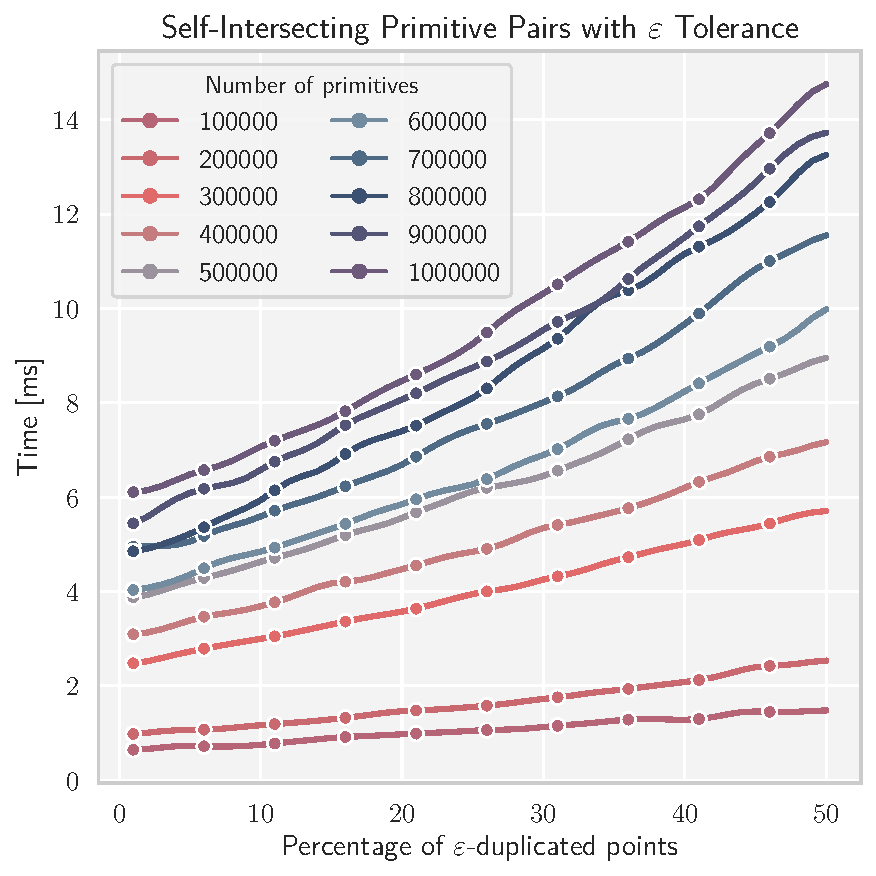
\includegraphics[width=\linewidth]{../figures/self_search_matrix.pdf}
\caption{
Performance of \texttt{tf::tree} on detecting $\varepsilon$-self-intersections.
Each curve corresponds to a point cloud of fixed size, with the x-axis indicating
the percentage of points duplicated and displaced by $\varepsilon$. The results
show that \texttt{tf::tree} maintains interactive self-query times even under
growing redundancy and scale.
}
\label{fig:self-search}
\end{figure}


\subsubsection{Collision Detection}

To assess collision detection performance, we sampled $10{,}000$
relative configurations between each model pair and checked for
collision in each case. Results show that the average time for
detecting a collision between two models is $47 \mu\mathrm{s}$. These values
are reported in Table~\ref{tab:tree-tree} under the
\textbf{collide} sub-heading.

In practice, we employ \texttt{tf::tree} for collision detection in
automatic model positioning pipelines, where models are
continuously checked for contact during iterative placement.

\subsubsection{Intersecting Primitive Pairs}

To evaluate the performance of \texttt{tf::tree} in computing
intersecting primitive pairs, we sampled $10{,}000$ relative
configurations resulting in intersection between each model pair.
For each sample, we computed all intersecting pairs of primitives.
The average evaluation times are reported in
Table~\ref{tab:tree-tree} under the
\textbf{intersect} sub-heading.

Our results show that \texttt{tf::tree} supports real-time
computation of intersecting primitive pairs (on the order of
milliseconds), even for large models. This capability forms the
foundation of our real-time mesh boolean pipeline, where fast and
reliable detection of intersections is the first step
\cite{sajovic2025trueform}.

\subsubsection{Self-Intersections with $\mathbf{\varepsilon}$ Tolerance}

To evaluate \texttt{tf::tree} on tolerant self-intersection detection,
we generated synthetic point clouds of varying sizes. For each size,
a percentage $p$ of points was duplicated and offset by $\varepsilon$
in a random direction—simulating geometric redundancy common in
real-world data.

The goal is to find all primitive pairs within $\varepsilon$ proximity,
i.e., all $\varepsilon$-self-intersections. These pairs guide merging
or deduplication, reducing the number of distinct points by roughly $p\%$.

As shown in Figure~\ref{fig:self-search}, \texttt{tf::tree} sustains
interactive self-query times even at large scales and high densities.

\subsection{Nearness Queries}

We evaluate the ability of \texttt{tf::tree} to efficiently compute
the closest point between two models across a wide range of
configurations. Given a pair of models, we first normalize them to
fit within a common bounding sphere. We then sample $10{,}000$
relative positions that result in an intersection, and for each
configuration, we compute the closest point using two different
strategies: a top-\emph{k} sorted stack and a standard priority queue.
The priority queue was implemented using a flat heap, employing the
\texttt{std::make\_heap}, \texttt{std::push\_heap}, and
\texttt{std::pop\_heap} functions of the standard \cpp library.

The results, averaged across all configurations, are reported in
Table~\ref{tab:tree-tree} under the \textbf{Nearness} heading.

\subsubsection{Top-K Stack}\label{sec:topk}

We evaluate the effectiveness of the top-\emph{k}
sorted stack strategy for nearness queries, which we configured
as specified in Section~\ref{sec:top-k}. Specifically, we compare
its runtime performance and the computational cost in terms of AABB
inspections against the baseline heap-based approach. The results
highlight the trade-off between increased traversal effort and
practical speed-up.

\begin{figure}[!t]
  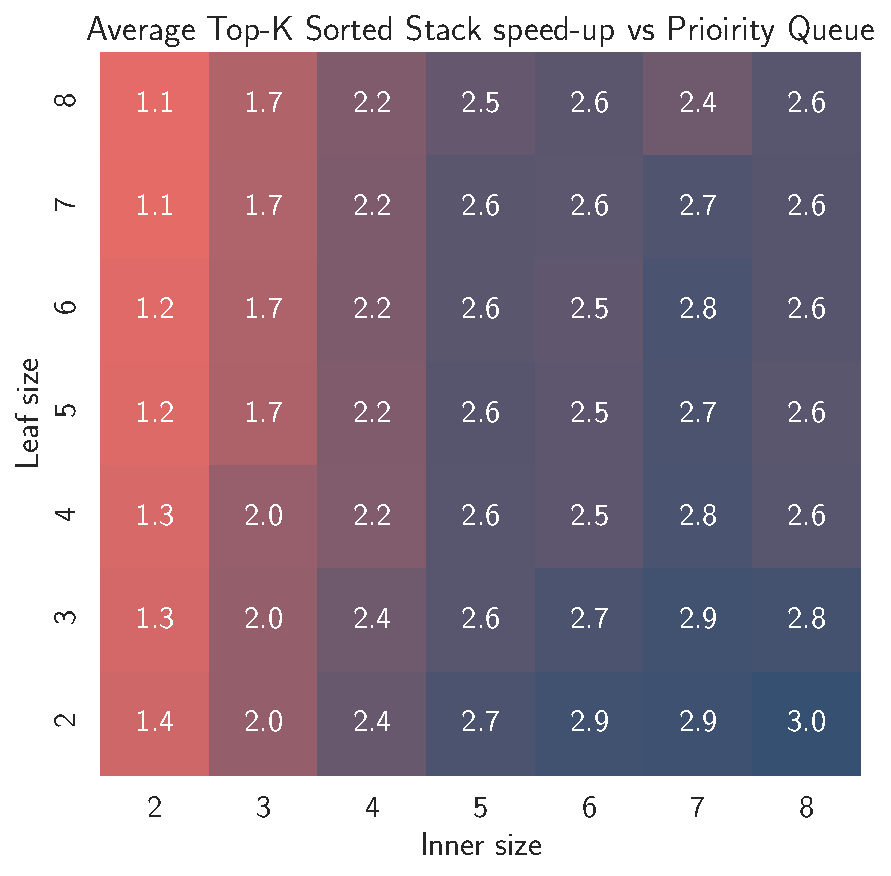
\includegraphics[width=\linewidth]{../figures/ftime-matrix.pdf}
\caption{
    Heatmap comparing the performance of Top-K Sorted Stack
    traversal versus Priority Queue for nearness queries across
    various tree configurations (varying tree arity and leaf size).
    The values represent the relative speed-up factor. Results
    indicate that the performance benefit of Top-K Sorted Stack
    increases with higher tree arity.}
  \label{fig:ftime-matrix}
\end{figure}



\paragraph*{AABB Inspections}

When using the top-\emph{k} sorted stack, \texttt{tf::tree} inspects
more AABBs during the search process compared to the heap-based
approach. This is expected: the partially sorted stack imparts approximate
ordering on the traverasal and does not prune optimally.
The increased number of inspections is quantified by the column
$\mathbf{f}^{\mathit{cost}}$, which reports the ratio of AABB
inspections between the top-\emph{k} sorted stack and the heap strategies.

Results show that the top-\emph{k} sorted stack performs $1.37\times$
AABB inspections as the priority queue based strategy.
Despite this increase, the sorted stack maintains a highly efficient
query structure by reducing traversal overhead and taking advantage
of cache-locality and simpler branching behavior.

\paragraph*{Peformance}

In practice, the top-\emph{k} sorted stack consistently outperforms
the heap-based alternative in terms of runtime. As shown in the
$\mathbf{f}_{\mathit{time}}$ column, it yields a speed-up factor
ranging from $1.7\times$ to over $3\times$ on complex models.
Furthermore, the performance benefit increases with
higher tree arity, as demonstrated in Figure~\ref{fig:ftime-matrix}.

While the heap strategy optimizes for minimal node visits, the
stack-based approach emphasizes speed through structural simplicity
and execution efficiency. These results demonstrate that even with
more geometric operations, the top-\emph{k} method provides
superior overall performance in practical applications.
